\documentclass[12pt]{article}
\usepackage{graphicx}
\usepackage{float}
\usepackage{amsmath}
\title{Experiment 5: Multiplier}
\author{Annirudh K P\\%
210070009}
\begin{document}

\maketitle

\section{Overview of the experiment}
\paragraph{}
In this experiment, we started working on more designs using structure modelling on VHDL. The problem statement of this experiment is to design a Multiplier, using the 4 Bit Adder already designed and other basic gates. The objective of this experiment was to understand the Quartus Design Flow, work with the Xen10 Board, and give us hands on experience over different technical glitches/problems we may face in this piece of software which has been made unwantedly hard.

\section{Experimental Set-up}

\subsection{Design Requirements}
\subsubsection{Multiplier}
The Multiplier takes in a 4 bit input and 3 bit input to spit out a 7 bit output. The functionality of multiplier is as shown.

\begin{figure}[H]
\centering
  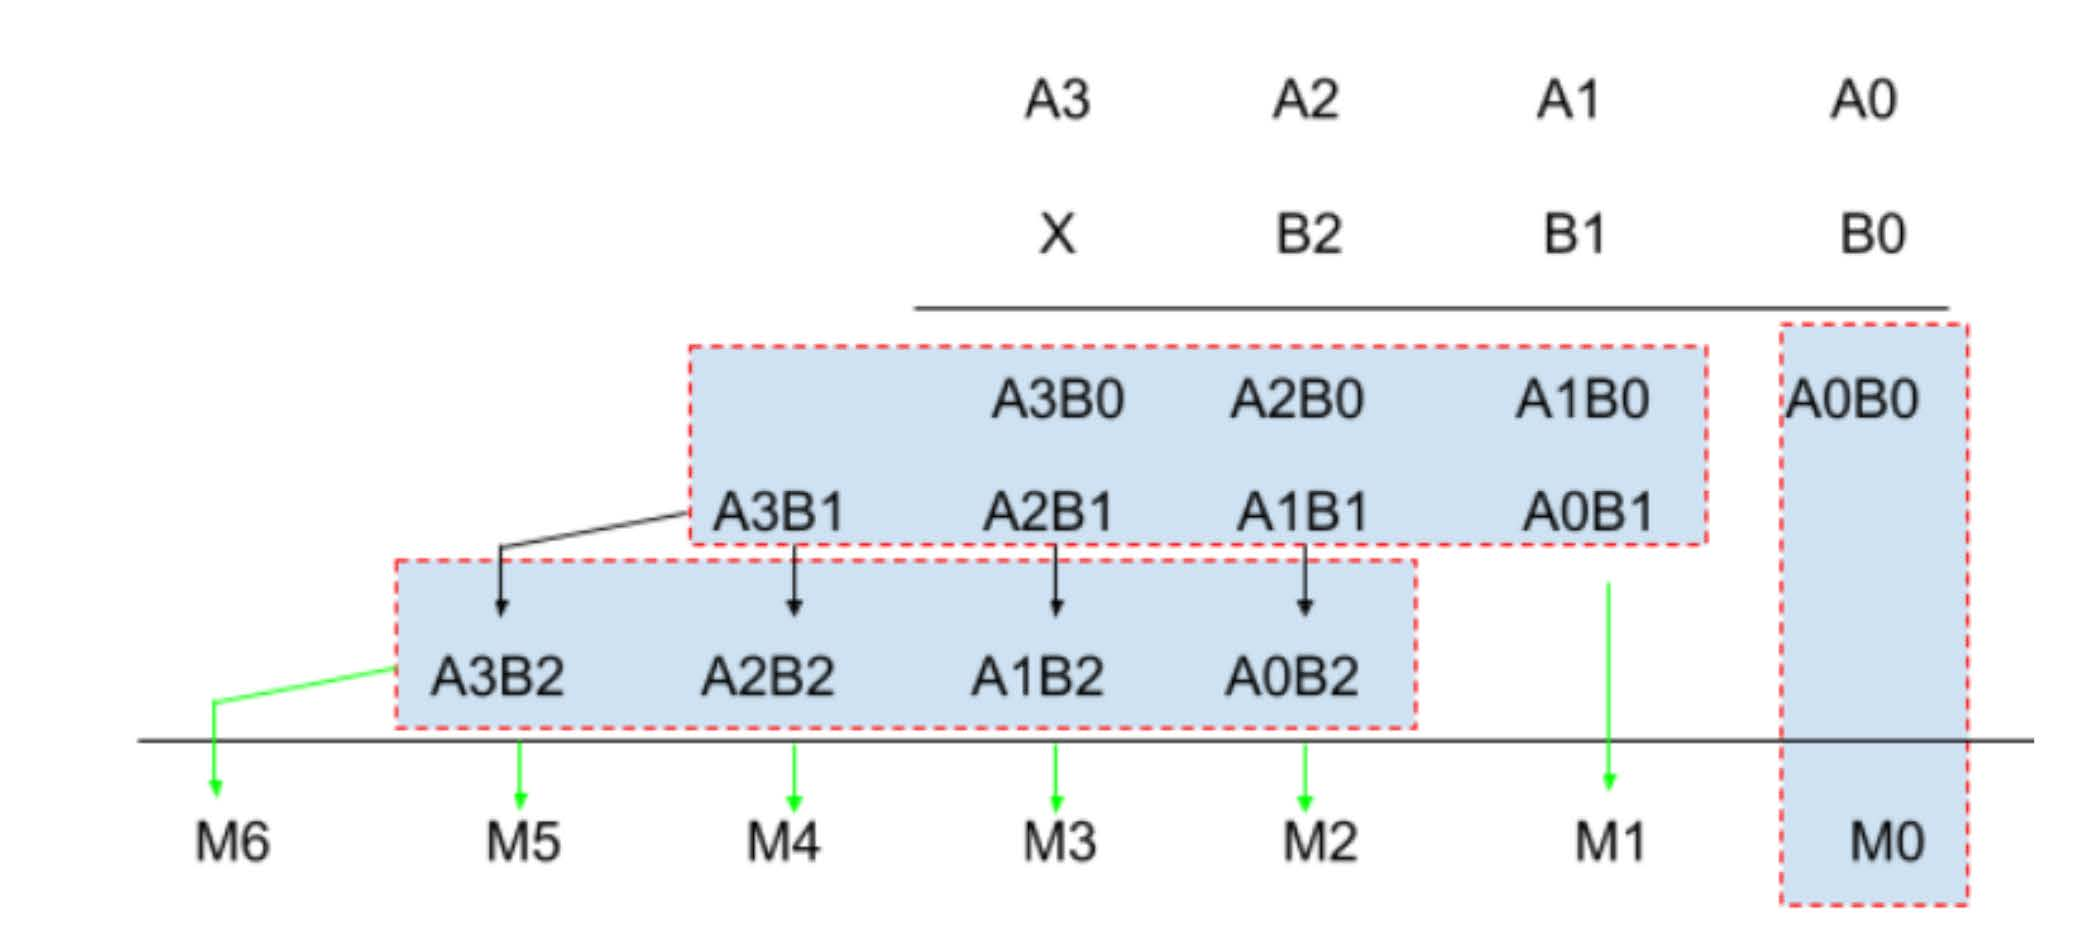
\includegraphics[scale=0.3]{Images/Multiplier_BlockDiagram.jpg}
  \caption{Multiplier Functionality}
\end{figure}


\subsection{Design Schematics}
The following design schematics are shown for the Multiplier 

\begin{figure}[H]
\centering
  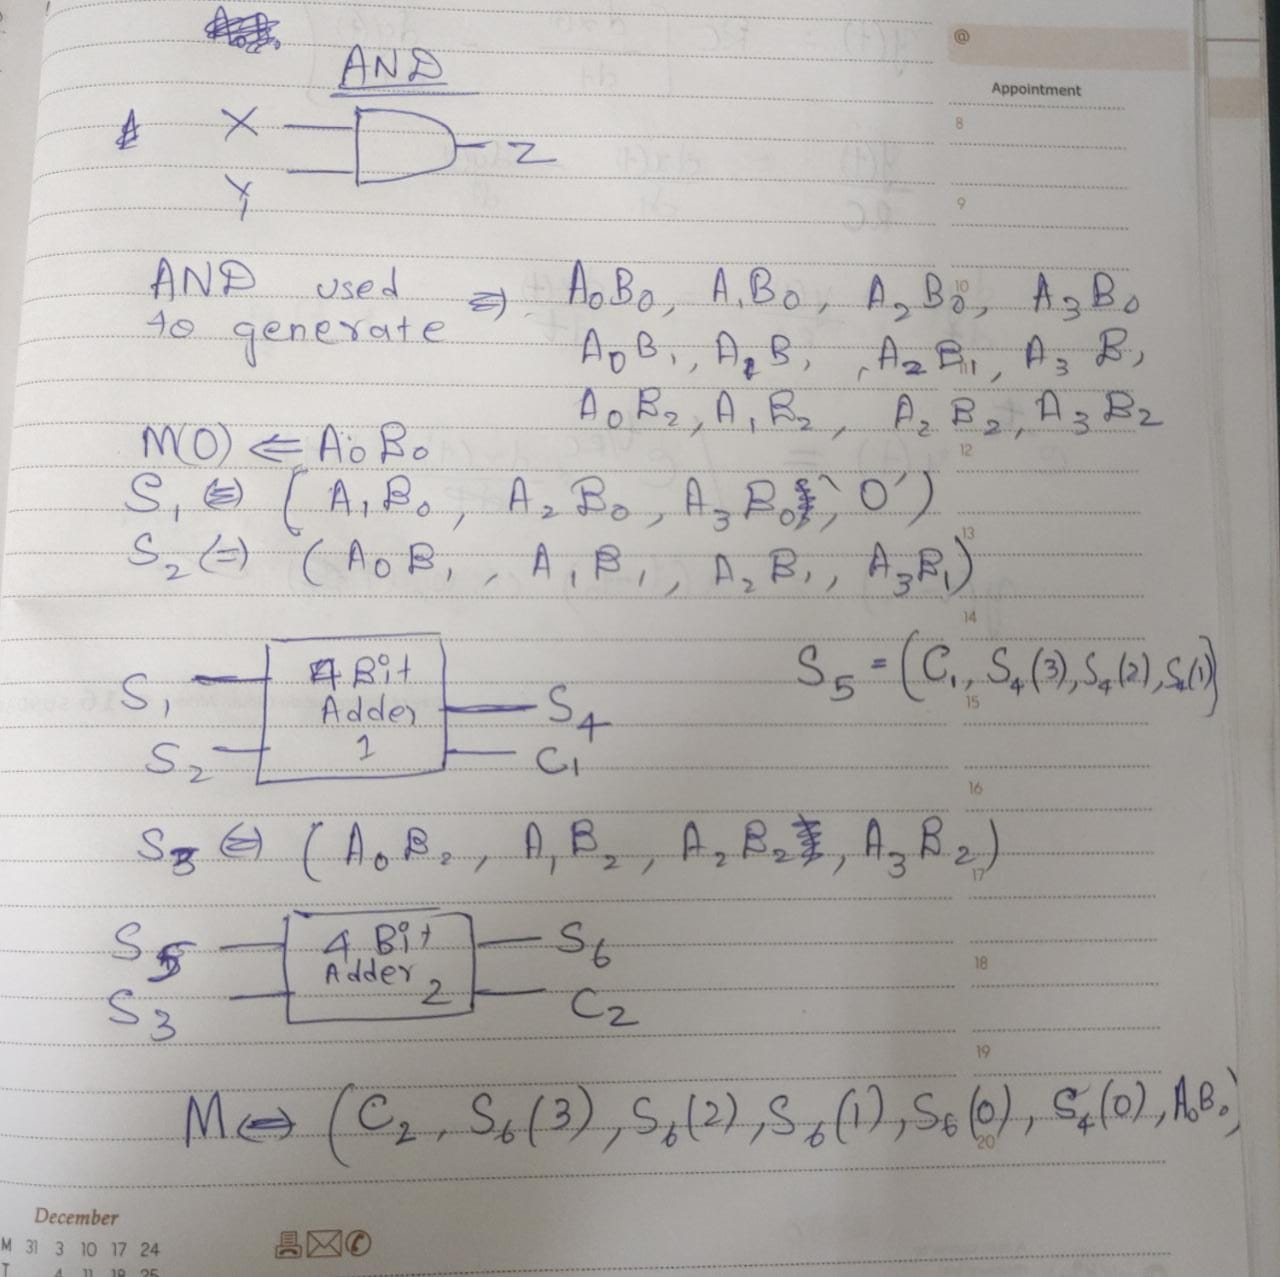
\includegraphics[scale=0.3]{Images/Multiplier_Design.jpeg}
  \caption{Multiplier Design}
\end{figure}

\begin{figure}[H]
\centering
  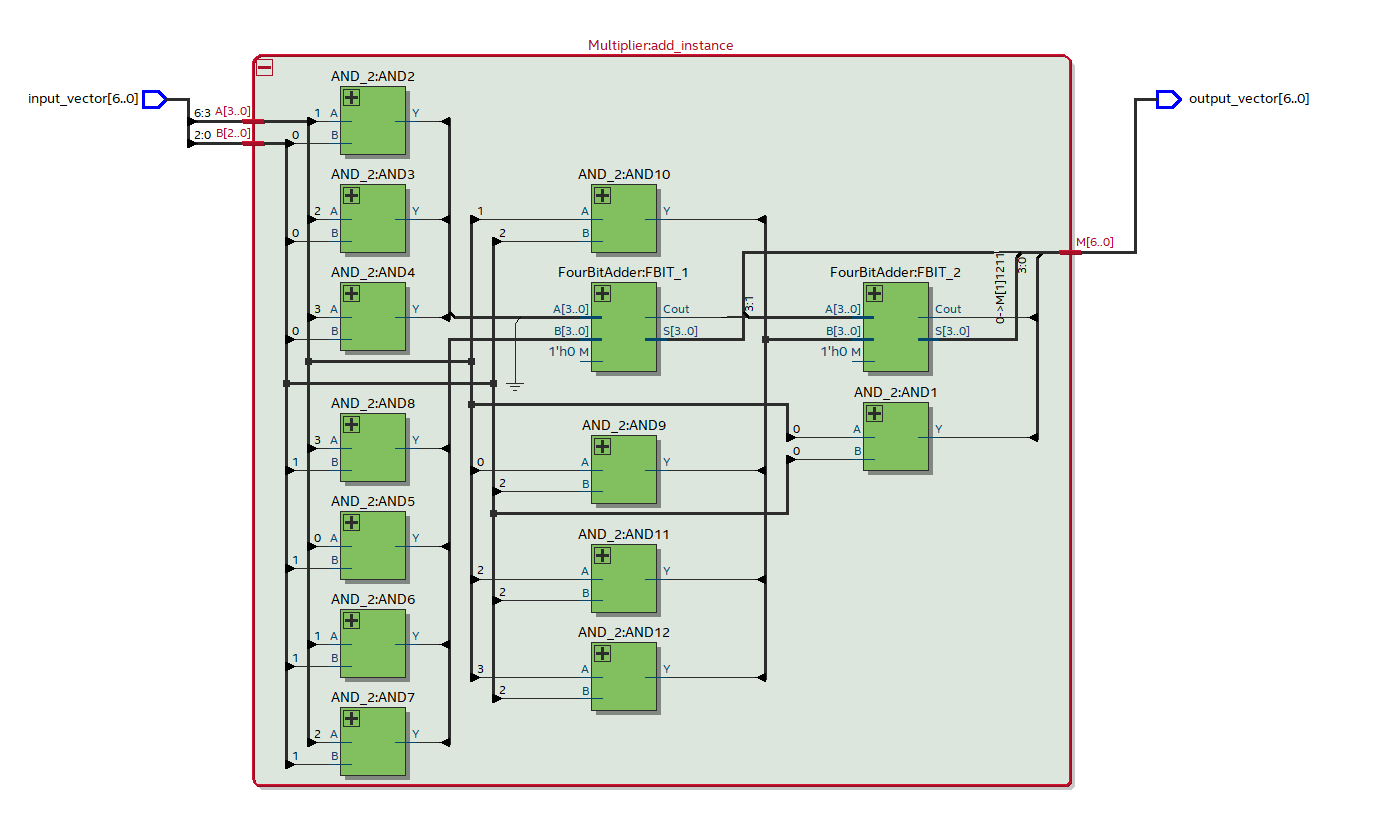
\includegraphics[scale=0.3]{Images/Multiplier_RTLViewer.png}
  \caption{Multiplier RTL View}
\end{figure}

\subsection{Description of Components}
\subsubsection{Multiplier}
\begin{verbatim}
library ieee;
use ieee.std_logic_1164.all;
library work;
use work.Gates.all;

entity OR_GATE  is
  port (A, B: in std_logic; OUTPUT: out std_logic);
end entity OR_GATE;

architecture Struct of OR_GATE is
	signal A_BAR, B_BAR : std_logic;
begin
  -- component instances
  NAND1: NAND_2 port map (A => A, B => A, Y => A_BAR);
  NAND2: NAND_2 port map (A => B, B => B, Y => B_BAR);
  
  -- final OR
  NAND3: NAND_2 port map (A => A_BAR, B => B_BAR, Y => OUTPUT);
end Struct;

library ieee;
use ieee.std_logic_1164.all;
library work;
use work.Gates.all;


entity HALF_ADDER1 is
	port (A, B: in std_logic; SUM, C0: out std_logic);
end entity HALF_ADDER1;

architecture Struct1 of HALF_ADDER1 is
	signal S1, S2, S3, S0 : std_logic;
begin
	--carry
	NAND1: NAND_2 port map (A => A, B => B, Y => S0);
	NAND2: NAND_2 port map (A => S0, B => S0, Y => C0);
	
	--sum
	NAND3: NAND_2 port map (A => A, B => B, Y => S1);
	NAND4: NAND_2 port map (A => A, B => S1, Y => S2);
	NAND5: NAND_2 port map (A => B, B => S1, Y => S3);
	NAND6: NAND_2 port map (A => S2, B => S3, Y => SUM);

end Struct1;

library ieee;
use ieee.std_logic_1164.all;
library work;
use work.Gates.all;

entity FULL_ADDER is
	port (A, B, CI: in std_logic; SUM, CO: out std_logic);
end entity FULL_ADDER;

architecture Struct2 of FULL_ADDER is
	signal S1, C1, C2 : std_logic;
	component HALF_ADDER1 is
		port (A, B: in std_logic; SUM, C0: out std_logic);
	end component HALF_ADDER1;
	component OR_GATE is
		port (A, B: in std_logic; OUTPUT: out std_logic);
	end component OR_GATE;
begin
	HA_1: HALF_ADDER1 port map (A => A, B => B, SUM => S1, C0 => C1);
	HA_2: HALF_ADDER1 port map (A => CI, B => S1, SUM => SUM, C0 => C2);
	OR_1: OR_GATE port map (A => C1, B => C2, OUTPUT => CO);
end Struct2;

library ieee;
use ieee.std_logic_1164.all;
library work;
use work.Gates.all;

entity XOR_GATE  is
  port (A, B: in std_logic; OUTPUT: out std_logic);
end entity XOR_GATE;

architecture Struct3 of XOR_GATE is
  signal S1, S2, S3 : std_logic;
begin
  -- component instances
  NAND1: NAND_2 port map (A => A, B => B, Y => S1);
  NAND2: NAND_2 port map (A => A, B => S1, Y => S2);
  NAND3: NAND_2 port map (A => B, B => S1, Y => S3);
  
  -- final XOR
  NAND4: NAND_2 port map (A => S2, B => S3, Y => OUTPUT);
  
end Struct3;

library ieee;
use ieee.std_logic_1164.all;
library work;
use work.Gates.all;

entity FourBitAdder  is
  port (M: in std_logic; A, B: in std_logic_vector(3 downto 0);
       	S: out std_logic_vector(3 downto 0); Cout: out std_logic); 
end entity FourBitAdder;

architecture Struct4 of FourBitAdder is
   signal Y1, Y2, Y3, Y4, Y5, Y6, Y7: std_logic;
	component XOR_GATE is
		port (A, B: in std_logic; OUTPUT: out std_logic);
	end component XOR_GATE;
	component FULL_ADDER is
		port (A, B, CI: in std_logic; SUM, CO: out std_logic);
	end component FULL_ADDER;
begin	
	XOR1: XOR_GATE port map (A => B(0), B => M, OUTPUT => Y1);
	FA_1: FULL_ADDER port map (A => Y1, B => A(0),  CI => M, 
		SUM => S(0), CO => Y2);
	XOR2: XOR_GATE port map (A => B(1), B => M, OUTPUT => Y3);
	FA_2: FULL_ADDER port map (A => Y3, B => A(1),  CI => Y2, 
		SUM => S(1), CO => Y4);
	XOR3: XOR_GATE port map (A => B(2), B => M, OUTPUT => Y5);
	FA_3: FULL_ADDER port map (A => Y5, B => A(2),  CI => Y4, 
		SUM => S(2), CO => Y6);
	XOR4: XOR_GATE port map (A => B(3), B => M, OUTPUT => Y7);
	FA_4: FULL_ADDER port map (A => Y7, B => A(3),  CI => Y6, 
		SUM => S(3), CO => Cout);
end Struct4;

library ieee;
use ieee.std_logic_1164.all;
library work;
use work.Gates.all;

entity Multiplier  is
  port (A: in std_logic_vector(3 downto 0);
			B: in std_logic_vector(2 downto 0);
       	M: out std_logic_vector(6 downto 0)); 
end entity Multiplier;

architecture Struct5 of Multiplier is
   signal S1, S2, S3, S4, S5, S6: std_logic_vector(3 downto 0);
	signal C1, C2: std_logic;
	component FourBitAdder  is
		port (M: in std_logic; A, B: in std_logic_vector(3 downto 0); 
		S: out std_logic_vector(3 downto 0); Cout: out std_logic); 
	end component FourBitAdder;
begin	
	AND1: AND_2 port map (A => A(0), B => B(0), Y => M(0));
	AND2: AND_2 port map (A => A(1), B => B(0), Y => S1(0));
	AND3: AND_2 port map (A => A(2), B => B(0), Y => S1(1));
	AND4: AND_2 port map (A => A(3), B => B(0), Y => S1(2));
	S1(3) <= '0';
	
	AND5: AND_2 port map (A => A(0), B => B(1), Y => S2(0));
	AND6: AND_2 port map (A => A(1), B => B(1), Y => S2(1));
	AND7: AND_2 port map (A => A(2), B => B(1), Y => S2(2));
	AND8: AND_2 port map (A => A(3), B => B(1), Y => S2(3));
	
	FBIT_1: FourBitAdder port map (M => '0', A => S1, B => S2, 
		S => S4, Cout => C1);
	M(1) <= S4(0); 
	S5(2 downto 0) <= S4(3 downto 1);
	S5(3) <= C1;
	
	AND9: AND_2 port map (A => A(0), B => B(2), Y => S3(0));
	AND10: AND_2 port map (A => A(1), B => B(2), Y => S3(1));
	AND11: AND_2 port map (A => A(2), B => B(2), Y => S3(2));
	AND12: AND_2 port map (A => A(3), B => B(2), Y => S3(3));
	
	FBIT_2: FourBitAdder port map (M => '0', A => S5, B => S3, 
		S => S6, Cout => C2);
	M(6) <= C2;
	M(5 downto 2) <= S6(3 downto 0);
	
end Struct5;
\end{verbatim}

\section{Observations}
 
We get RTL simulation waveforms for corresponding to input and output which is given below and it shows required results.

\begin{figure}[H]
\centering
  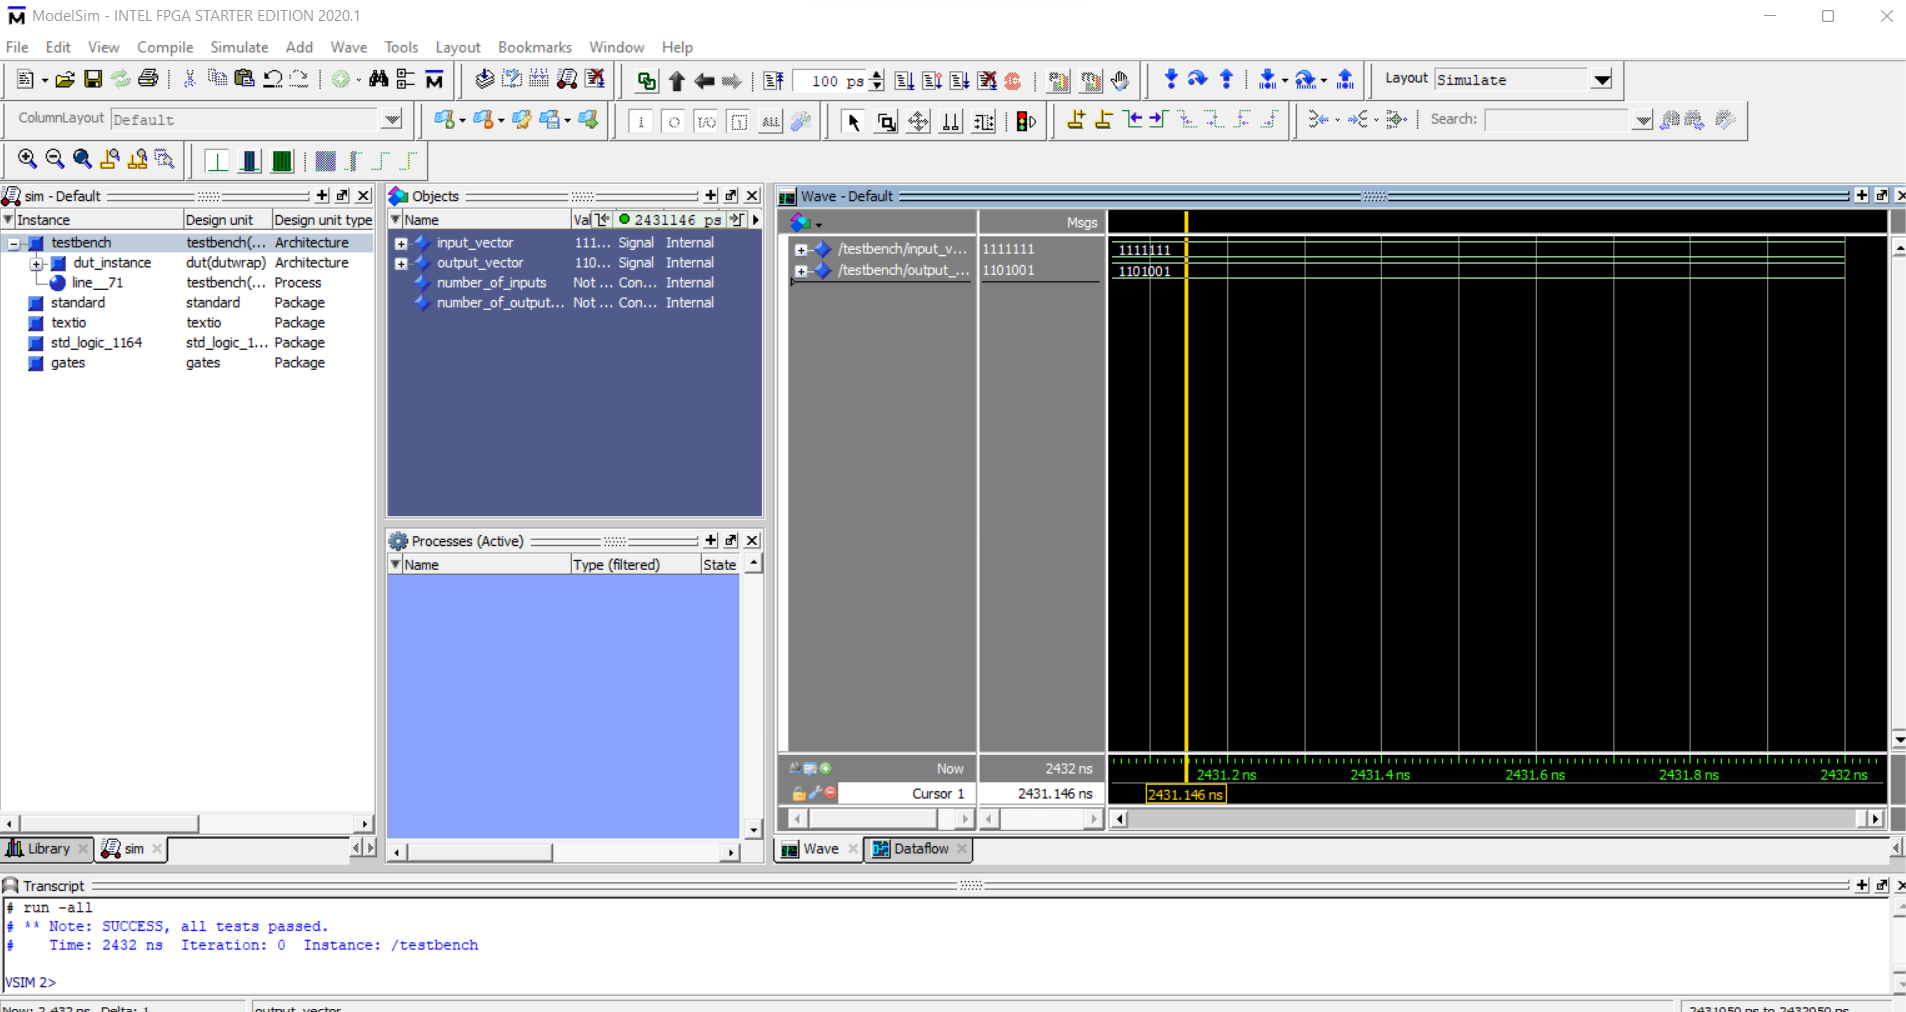
\includegraphics[scale=0.35]{Images/Multiplier_RTLSimulation.png}
  \caption{Multiplier RTL Simulation Waveform}
\end{figure}

Further the code (in form of .svf file) was flashed onto the Xen10 board. Then scanchain was run to generate outputs using tracefile and then compared to the golden outputs to check if the outputs were indeed correct. The output was verified, which also verified the working of the logic for the Multiplier. The output file's content is shown below.

\begin{verbatim}
0000000 0000000 Success
0000001 0000000 Success
0000010 0000000 Success
0000011 0000000 Success
0000100 0000000 Success
0000101 0000000 Success
0000110 0000000 Success
0000111 0000000 Success
0001000 0000000 Success
0001001 0000001 Success
0001010 0000010 Success
0001011 0000011 Success
0001100 0000100 Success
0001101 0000101 Success
0001110 0000110 Success
0001111 0000111 Success
0010000 0000000 Success
0010001 0000010 Success
0010010 0000100 Success
0010011 0000110 Success
0010100 0001000 Success
0010101 0001010 Success
0010110 0001100 Success
0010111 0001110 Success
0011000 0000000 Success
0011001 0000011 Success
0011010 0000110 Success
0011011 0001001 Success
0011100 0001100 Success
0011101 0001111 Success
0011110 0010010 Success
0011111 0010101 Success
0100000 0000000 Success
0100001 0000100 Success
0100010 0001000 Success
0100011 0001100 Success
0100100 0010000 Success
0100101 0010100 Success
0100110 0011000 Success
0100111 0011100 Success
0101000 0000000 Success
0101001 0000101 Success
0101010 0001010 Success
0101011 0001111 Success
0101100 0010100 Success
0101101 0011001 Success
0101110 0011110 Success
0101111 0100011 Success
0110000 0000000 Success
0110001 0000110 Success
0110010 0001100 Success
0110011 0010010 Success
0110100 0011000 Success
0110101 0011110 Success
0110110 0100100 Success
0110111 0101010 Success
0111000 0000000 Success
0111001 0000111 Success
0111010 0001110 Success
0111011 0010101 Success
0111100 0011100 Success
0111101 0100011 Success
0111110 0101010 Success
0111111 0110001 Success
1000000 0000000 Success
1000001 0001000 Success
1000010 0010000 Success
1000011 0011000 Success
1000100 0100000 Success
1000101 0101000 Success
1000110 0110000 Success
1000111 0111000 Success
1001000 0000000 Success
1001001 0001001 Success
1001010 0010010 Success
1001011 0011011 Success
1001100 0100100 Success
1001101 0101101 Success
1001110 0110110 Success
1001111 0111111 Success
1010000 0000000 Success
1010001 0001010 Success
1010010 0010100 Success
1010011 0011110 Success
1010100 0101000 Success
1010101 0110010 Success
1010110 0111100 Success
1010111 1000110 Success
1011000 0000000 Success
1011001 0001011 Success
1011010 0010110 Success
1011011 0100001 Success
1011100 0101100 Success
1011101 0110111 Success
1011110 1000010 Success
1011111 1001101 Success
1100000 0000000 Success
1100001 0001100 Success
1100010 0011000 Success
1100011 0100100 Success
1100100 0110000 Success
1100101 0111100 Success
1100110 1001000 Success
1100111 1010100 Success
1101000 0000000 Success
1101001 0001101 Success
1101010 0011010 Success
1101011 0100111 Success
1101100 0110100 Success
1101101 1000001 Success
1101110 1001110 Success
1101111 1011011 Success
1110000 0000000 Success
1110001 0001110 Success
1110010 0011100 Success
1110011 0101010 Success
1110100 0111000 Success
1110101 1000110 Success
1110110 1010100 Success
1110111 1100010 Success
1111000 0000000 Success
1111001 0001111 Success
1111010 0011110 Success
1111011 0101101 Success
1111100 0111100 Success
1111101 1001011 Success
1111110 1011010 Success
1111111 1101001 Success
\end{verbatim}

\end{document}